\chapter{Conclusión}
Este proyecto trata de buscar una solución simple para la detección de arritmias de una señal de un electrocardiograma, Para la elaboración de este proyecto, 
se ha estudiado el comportamiento de las arritmias, viendo la base de datos de MIT y estudiando el comportamiento de las arritmias anotadas se observó que la inmensa mayoría de las arritmias que ocurrían eran dadas por una contracción prematura del corazón, por tanto el proyecto, aunque inicialmente se pensó detectar el mayor tipo de arritmias posibles, al no ver ningún ejemplo claro de arritmia no producida por una contracción prematura el proyecto solo se centró en detectar dichas arritmias.

Se realizó un prototipo en \textit{python} que sirvió para crear el algoritmo y probarlo con facilidad. Este prototipo inicia
con un filtrado de la señal original aplicando el filtrado FIR. Seguidamente se aplica un algoritmo de detección de 
picos QRS sobre la señal filtrada que busca el pico más alto que además sobrepase el \textit{cutoff} dinámico establecido. Finalmente
se aplica el algoritmo de detección de arritmias calculando la distancia entre el pico actual con el anterior y comparándola con una
distancia anterior de un ritmo normal.

Para la implementación de  \textit{hardware}  se utilizaron 3 módulos principales que son el módulo de filtrado, el módulo de detección de picos 
y el módulo de detección de arritmias. Además estos módulos están contenidos en un módulo principal. Para hacer las pruebas sobre
estos módulos, se añaden 2 módulos adicionales de input de señal y output donde se comparan los resultados de las anotaciones. Además 
se evalúan los resultados mediante una simulación al crear un \textit{testbench}.

Para las pruebas en  \textit{hardware}  se utiliza la FPGA \textit{Artix 7} en la placa \textit{Basys3}, ya que es la FPGA que se usa en el estudio y aunque no sea capaz de albergar los 30 minutos de pruebas en la RAM, con menos pruebas tiene un buen desempeño.

En el fichero .xdc se ha establecido un periodo específico teniendo en cuenta la frecuencia de las muestras que es de 360 sps y da un periodo de 1852 ns. Gracias al reporte de \textit{timing} se halla que el mínimo periodo de funcionamiento es de 6,49 ns.

Según el reporte de potencia el consumo de la placa es de 0,069 vatios, y solamente el algoritmo consume menos de 0,001 vatios, lo que resulta en un consumo bajo incluso para un uso continuo de este. Comparándolo con otros proyectos similares, el consumo dinámico es menor.

\chapter{Trabajo futuro}

Como trabajo futuro, se ha propuesto sincronizar el proyecto con un dispositivo capaz de detectar latidos del corazón para mostrar pruebas en tiempo real y demostrar la eficacia del proyecto en cualquier persona. Además, se considera la posibilidad de implementar todo lo anterior en un dispositivo similar a un reloj para crear un producto que cumpla todos los objetivos mencionados en el proyecto.

También se ha pensado en realizar un trabajo de investigación para explorar alternativas en el ámbito médico y compararlas en términos de consumo y eficacia. Este trabajo de investigación proporcionaría información valiosa para mejorar y optimizar el proyecto actual, así como para identificar oportunidades para futuras investigaciones y desarrollos.

Por último, se ha contemplado la posibilidad de ampliar el proyecto para detectar más tipos de arritmias siguiendo los patrones que estas presentan, lo que permitiría desarrollar un algoritmo más completo y versátil para la detección de arritmias cardíacas.

\chapter*{Conclusion}

This project tries to find a simple solution for the detection of arrhythmias from an electrocardiogram signal, For the development of this project, 
The behavior of arrhythmias has been studied, looking at the MIT database and studying the behavior of the annotated arrhythmias it was observed that the vast majority of arrhythmias that occurred were given by a premature contraction of the heart, therefore the project, although initially it was thought to detect the largest possible type of arrhythmias, not seeing any clear example of arrhythmia not produced by a premature contraction made the project only to focus on detecting these arrhythmias.

A prototype was made in python which was used to create the algorithm and test it easily. This prototype starts with a filtering of the original signal by applying FIR filtering. Next, a QRS peak detection algorithm is applied to the filtered signal, searching for the highest peak that also exceeds the established dynamic cutoff. Finally the arrhythmia detection algorithm is applied by calculating the distance between the current peak and the previous peak and comparing it with a previous distance of a normal rhythm.

For the hardware implementation, 3 main modules were used, which are the filtering module, the peak detection module and the arrhythmia detection module. In addition these modules are contained in a main module. In order to test on these modules. These modules are tested by adding 2 additional modules for signal input and output where the results of the annotations are compared. Furthermore the results are evaluated by means of a simulation when creating a testbench.

For the tests on hardware the FPGA Artix 7 on the Basys3 board is used, since it is the FPGA used in the study and although it is not able to hold the 30 minutes of tests in RAM, with fewer tests it performs well.

In the .xdc file a specific period has been established taking into account the frequency of the samples which is 360 sps and gives a period of 1852 ns. Thanks to the timing report it is found that the minimum operating period is 6.49 ns.

According to the power report the power consumption of the board is 0.069 watts, and only the algorithm consumes less than 0.001 watts, which results in a low power consumption even for a continuous use of the algorithm. Compared to other similar projects, the dynamic power consumption is lower.

\chapter*{Introduction}
\section*{Arrhythmia concept}
Cardiovascular diseases are the leading cause of death in the world \cite{roth2020global} and one of the most common causes of these diseases is arrhythmias.

A cardiac arrhythmia is a result of a disturbance in the initiation or propagation of the heart's rhythm \cite{velez}. If an arrhythmia occurs, the heart may have a rhythm that is too fast, too slow or irregular. This can cause symptoms such as palpitations, dizziness, shortness of breath and even fainting, all of these can become life-threatening.

Cardiologists use devices such as a Holter\footnote{\textbf{Holter}:A portable medical device used to monitor and record the electrical activity of the heart over an extended period of time} to generate electrocardiograms (ECGs), which are diagrams that represent the heartbeat, and with them they are able to analyze and find cardiac abnormalities.

Among these anomalies are premature contractions of the heart, a type of arrhythmia that this project will detect. 

\begin{figure}[h!]
	\centering
	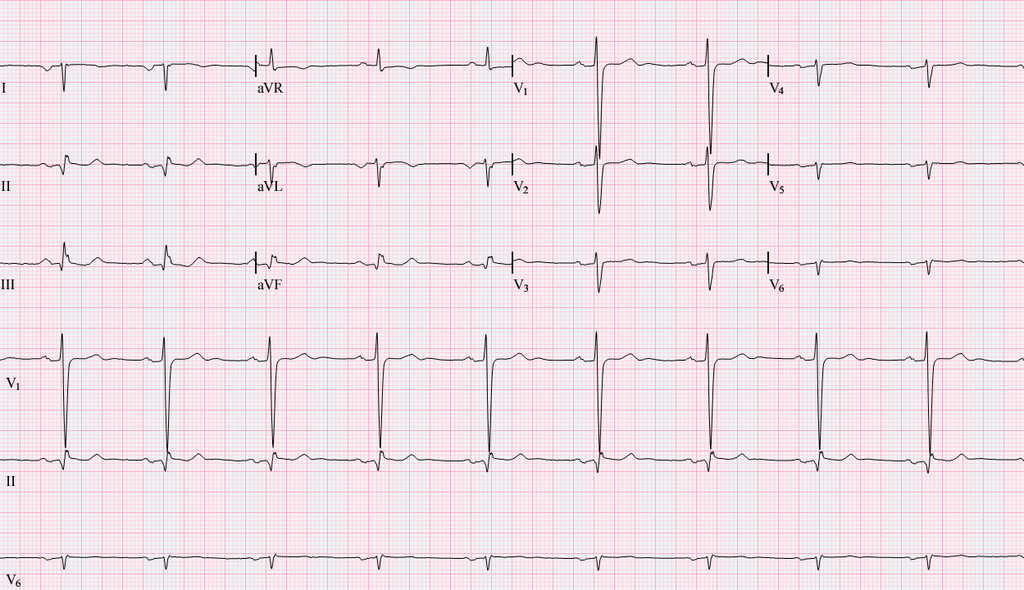
\includegraphics[width=0.7\textwidth]{./Images/img_introduccion/electrocardiograma.png}
	\caption{Image of several electrocardiograms generated by a Holter \textit{Holter} \cite{fotoElectrocardiograma}}.
	\label{fig:electrocardiogramas}
\end{figure}

\section*{Detection algorithm}
The arrhythmia detection algorithm used in this project is based on the detection of the QRS peaks produced in the electrocardiogram. 
QRS peaks produced in the electrocardiogram.

A QRS spike, as shown in the \Cref{fig:complejoQRS}, on an electrocardiogram is caused by the contraction of the ventricle as it pumps blood through the arteries. This is the strongest electrical impulse that the heart produces in each beat \cite{wiki:complejoQRS}. In this project we will use these peaks to compare the distance between them to determine if an arrhythmia has occurred. 

\begin{figure}[h]
	\centering
	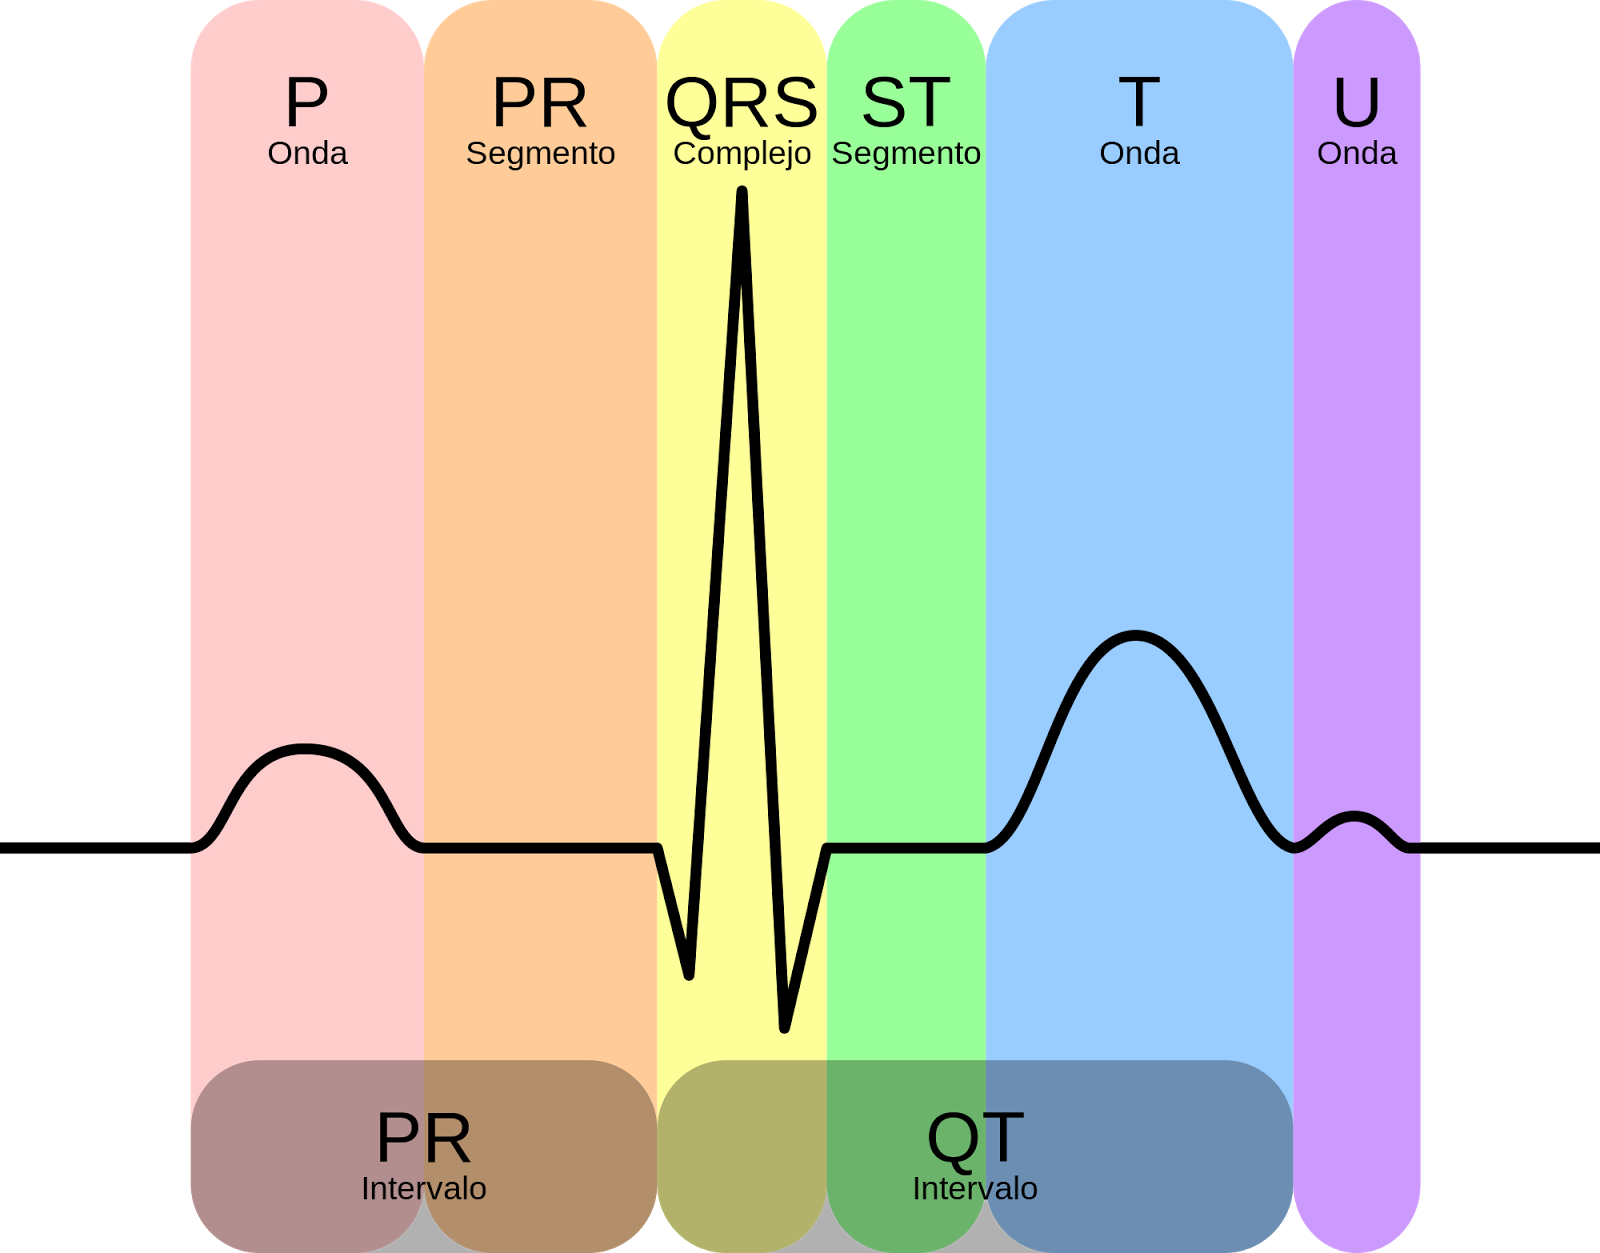
\includegraphics[width=0.4\textwidth]{./Images/img_introduccion/complejoQRS.png}
	\caption[Complejo QRS]{QRS Complex \cite{desai2021low}}
	\label{fig:complejoQRS}
\end{figure}

This algorithm is of particular interest\cite{kiranyaz2011personalized} because the development of efficient techniques to automate ECG analysis is essential to assist cardiologists in their diagnoses, especially in the detection of arrhythmias. The cardiologist would have to spend several minutes to find arrhythmias in an ECG of, for example, 30 minutes. This algorithm is not intended to be a definitive solution for the detection of arrhythmias, as several years of study are required to fully understand them. Therefore, it focuses on detecting premature ventricular contractions.

\subsection*{Filtrado}
As it can be seen in the \Cref{fig:102filtradoysinfiltrar} it is convenient to filter the rhythm strips in order to better detect the QRS peaks, since filtering centers the signal wave on the 0 value and avoids failures in the peak detection algorithm, which will be discussed later. 

In the creation of the project we have tried not to filter the waveform to check if better results are obtained than without such filtering, but this has not been the case due to the irregularities of the waveform.

\begin{figure}[h!]
	\centering
	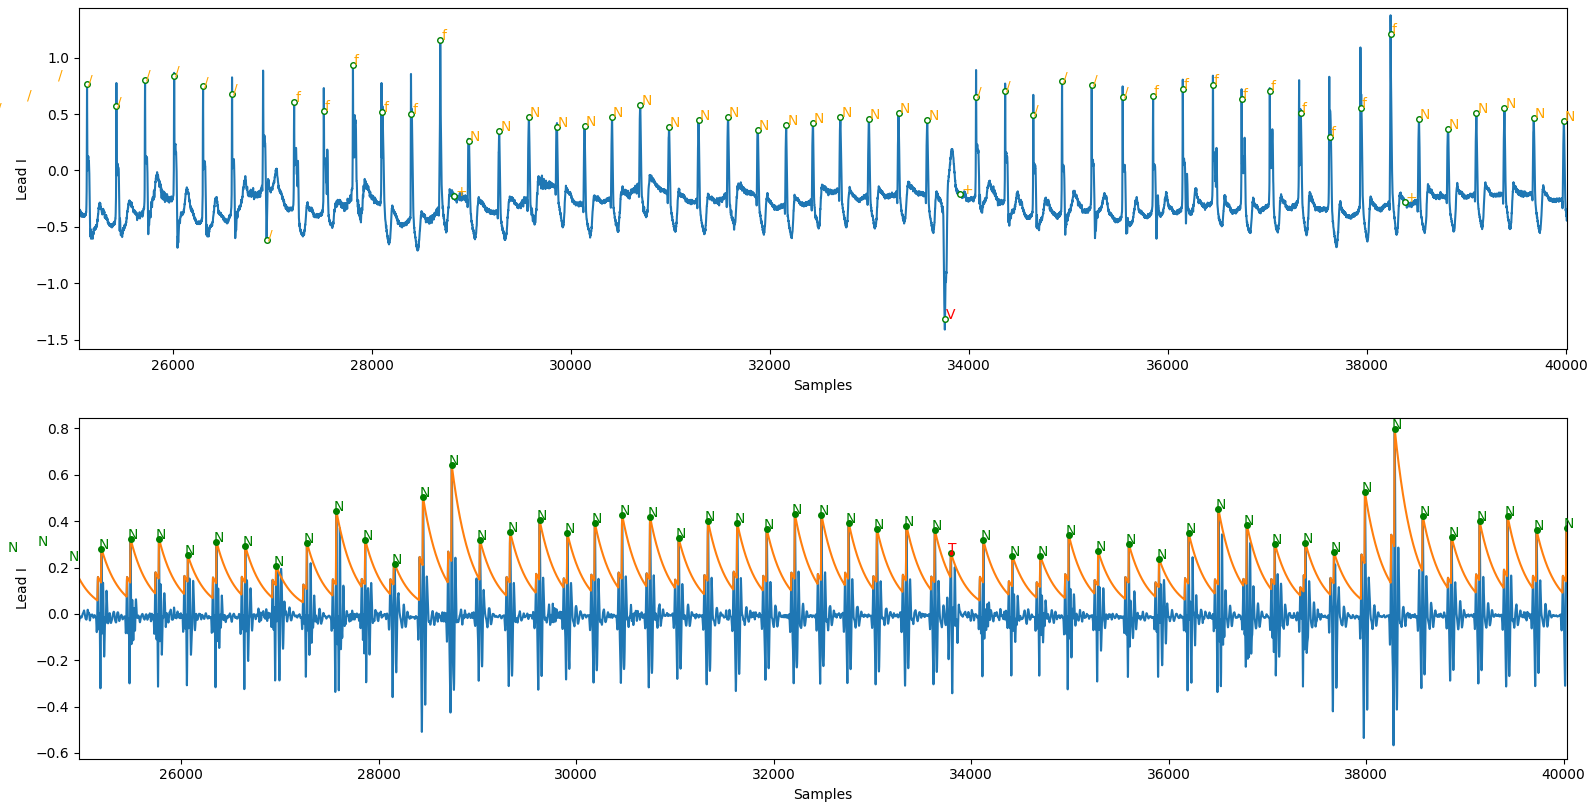
\includegraphics[width=0.99\textwidth]{./Images/img_introduccion/102filtrado_y_sin_filtrar.png}
	\caption{Example of an original electrocardiogram and a filtered one of patient 102}
	\label{fig:102filtradoysinfiltrar}
\end{figure}

\section*{Reference data}
The reference data for testing the algorithm were obtained from a study conducted at the Massachusetts Institute of Technology (MIT)\cite{MIT} in which half-hour tests were performed on a number of patients of varying ages, some of whom were implanted with pacemakers.

The data consist of electrocardiograms that have previously been analyzed by cardiologists and whose annotations indicate when a patient has suffered an arrhythmia, when the rhythm is normal and when there has been a failure in the reading of the signal, as seen in \cref{fig:Paciente_pruebas_MIT}. Less relevant information for our study is also shown, such as when an error has occurred. study, such as when there has been an error in the signal reading and pacemaker activation.\footnote{\textbf{Pacemaker}: A device implanted in the heart that acts when the heart is not pumping blood strongly enough, i.e. the QRS peak is not as prominent and the help of such a device is needed to provide the necessary electrical impulse.}.

\begin{figure}[h]
	\centering
	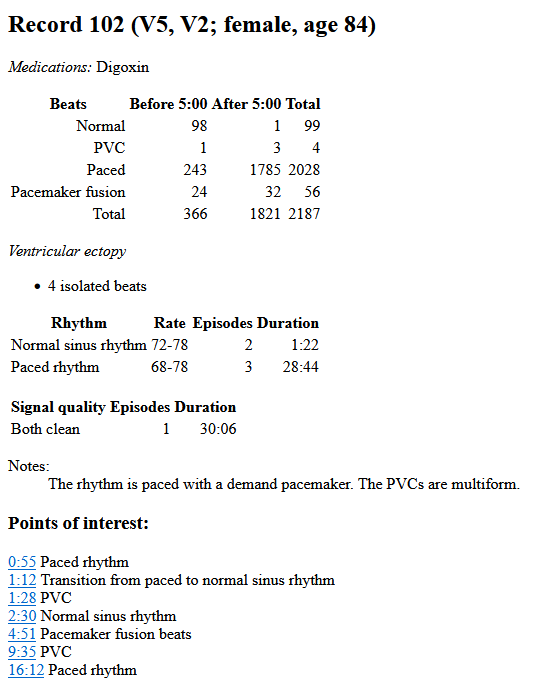
\includegraphics[width=0.6\textwidth]{./Images/img_introduccion/Paciente_pruebas_MIT.png}
	\caption{Example with patient 102 \cite{mitdb}}
	\label{fig:Paciente_pruebas_MIT}
\end{figure}

\section*{Use of FPGAs}
This algorithm has been designed to run on a small, lightweight and portable device, which is why it is convenient to run it on an FPGA \cite{mdpi_sensors_2014}. This is because there are small FPGAs that have enough hardware to be able to execute this algorithm, in addition the consumption produced by an FPGA when executing this algorithm is quite low as will be shown later.

For this project we used the Artix-7 FPGA \cite{xilinx_artix7} on the Basys3 board to test the operation of the algorithm. However, for testing, due to the amount of test values pulled from the database per patient, it was considered to use another FPGA whose hardware can support such amount of data.


\section*{Project objectives}

The main objective of the project is to create an algorithm based on the study of signal characterization using Hermite polynomial \cite{desai2021low} that detects arrhythmias in patients and that this algorithm is capable of running on a portable device, which has low power consumption and works in real time. In order to achieve the main objective, it is necessary to achieve a series of objectives which are as follows:

\begin{enumerate}
    \item Finding out what arrhythmias are, how they occur, what arrhythmias the program could detect and what pattern most of them follow.
    \item The creation of a software algorithm capable of reading and filtering the original signal of the patients in the database, the creation of an algorithm to detect the peaks where ventricular contraction occurs as they appear in the filtered signal and, finally, the creation of an algorithm to detect the arrhythmias according to the pattern found in the previous objective.
    \item The replication of the program in hardware according to the prototype previously created in software. Using the necessary hardware for the algorithm to work in an FPGA and the necessary hardware to be able to test in simulation and on the board.
    \item The observation of the experimental results of the amount of resources used, the resources used by the algorithm and the time it takes to be carried out according to the arrival of the patient's signal. These experimental results should be consistent with the main objective.
\end{enumerate}


\section*{Work plan}
\begin{enumerate}
	\item Research and theoretical basis:
	
	\begin{enumerate}
		\item Review the book\cite{velez} and consult with a first aid medic to understand what arrhythmias are and how they occur.
	
		\item Use the information obtained to establish the medical basis for the project.
	\end{enumerate}

	\item Data collection and preparation:
	\begin{enumerate}
		\item Locate and download the project database used in the signal characterization study using Hermite polynomials. \cite{desai2021low}.

		\item Represent the signals in Python and perform the filtering as described in the aforementioned study.
	\end{enumerate}
	\item Algorithm Development:
	\begin{enumerate}
		\item Implement the QRS peak detection algorithm and the arrhythmia detection algorithm.

		\item Perform tests and adjustments to the algorithms to obtain satisfactory results.
	\end{enumerate}
	
	\item Hardware implementation: 
	\begin{enumerate}
		\item Design the main modules for each part of the algorithm: peak detection, arrhythmia detection, filtering and a main module.

		\item Create additional modules to perform simulations in Vivado and verify program performance.
		\item Develop a testbench to generate the clock frequency and signals needed to simulate the system.
	\end{enumerate}

	\item Analysis of experimental results:
	\begin{enumerate}
		\item Evaluate the results obtained from the analyses performed at Vivado.

		\item Draw relevant conclusions to the project objectives.
	\end{enumerate}
\end{enumerate}

\section*{Algorithm analysis and optimization}
The algorithm focuses on three main functions:
\begin{enumerate}
	\item Filtering of the original signal: FIR filtering is used\cite{FIR}, which makes the signal easier to process to find the QRS peaks. This is done by multiplying the original signal values by the filter coefficients stored in a memory.
	\item Peak detection on the filtered signal: Each value of the filtered signal is analyzed and if that value is higher than its previous values, it is considered a possible peak. If after 72 values it remains as the highest value, then that value is considered a QRS peak. Additionally, a dynamic cutoff is established in which, if the signal peaks do not exceed that value, they are not taken into account.
	\item Arrhythmia detection by comparing the position of the peaks: Once the QRS peaks are obtained, the distance of the current peak from the previous peak is calculated and, depending on the previous distances, it is determined if there is an arrhythmia.
\end{enumerate}

\section*{FPGA Implementation}
To implement the code in the FPGA, several modules will be implemented, which generally try to replicate the functionalities performed by the software algorithm and will become the most important part of the program.  

The main modules are.

	\begin{enumerate}
		\item Filtering module: The filter coefficients are stored in a ROM memory module and the values of the original signal in a RAM memory, then each sample is multiplied by its corresponding coefficient and the result is accumulated. Once the multiplication and accumulation process is finished, the calculated value is transmitted to the next main module.
		\item Peak detection module on the filtered signal: A finite state machine is implemented which analyzes each value of the filtered signal and calculates if it is a possible peak, or a QRS peak. As the signal values are real numbers, several modules are implemented to be able to operate with the signal values in floating point. 
		\item Arrhythmia detection module: A finite state machine is implemented to receive a QRS peak as input, store the most recent distances, determine if an arrhythmia has occurred according to the difference of these distances, and display a flag as output.
	\end{enumerate}
	
	In addition to these modules, a main module must be created to encapsulate them and a testbench module to test the operation of the program with the signals from the database. \cite{desai2021low}.

\section*{Organization of the memory}
Chapter 2 will show how the algorithm was prototyped in software. Section 2.1 shows the course of the algorithm. In section 2.2, the libraries used for data collection will be shown. In section 2.3, the type of filtering used for the original signal will be explained. In section 2.4, the QRS peak detection algorithm and the methodologies followed will be presented. In section 2.5, the arrhythmia detection algorithm will be explained and in section 2.6, the algorithm for testing the prototype and obtaining statistics of the tests performed.

In chapter 3, the different modules created for the hardware implementation will be discussed. In section 1, the modules for floating-point operations and the memories used will be specified. From section 2 to 4, the operation of the signal filtering module, the peak detection module and the arrhythmia detection module will be explained. In section 5, the creation of the main module and the used testbench will be discussed.

In chapter 4, the experimental results obtained will be shown, such as the FPGA used, hardware utilization analysis, timing analysis and consumption.

Finally, in chapter 5, a conclusion will be given on this project and future work will be suggested in case there is a desire to extend the project.